%
% LaTeX template for Student Thesis & PhD Thesis
%
% Institute of Biomedical Engineering
% Karlsruhe Institute of Technology (KIT)
% www.ibt.kit.edu
%
% IBT template v1.1 (2016-04-26)
% Developed by Thomas Fritz & Axel Loewe based on the memoir class

%%%%%%%%%%%%%%%%%%%%%%%%%%%%%%%%%%%%%
%%%%%%%%%%% CONFIGURATION %%%%%%%%%%%
%%%%%%%%%%%%%%%%%%%%%%%%%%%%%%%%%%%%%

% How does it work?
% \newif\ifmyvariable will create a variable called myvariable and set is to 
% false.  In order to set it to true, use \myvariabletrue

%%% Language of thesis
\newif\ifenglish 
% \englishtrue % define if thesis is in English

%%% Citation style
\newif\ifapa
% \apatrue             % define if APA style references are desired (Courtemanche et al., 2013)

%%% List of figures and tables
\newif\iflists
% \liststrue            % define if you want to include a list of figures and a lists of tables

%%% PhD Thesis or Student Thesis
\newif\ifthesisIsDiss
% \thesisIsDisstrue      % define for PhD Thesis

\ifthesisIsDiss
  %%% PhD Thesis for preparation or book print
  \newif\ifdissForPrint
    \dissForPrinttrue   % define Print Process at KIT Scientific Publishing (only affects title page)
\fi

%%% Paper format A5
\newif\ifafive
% \afivetrue

%%% License necessary for the publication at KITopen.
\newif\iflicense
\licensetrue  % enable license

\newif\ifsharealike 
\sharealiketrue %   Creative Commons Attribution – Share Alike 4.0 International License

%%%%%%%%%%%%%%%%%%%%%%%%%%%%%%%%%%%%%
%%%%%%%%% END CONFIGURATION %%%%%%%%%
%%%%%%%%%%%%%%%%%%%%%%%%%%%%%%%%%%%%%

\ifafive
  \documentclass[10pt,final,openright,a5paper]{memoir}
  %\usepackage[a5paper,hcentering,bindingoffset=0.5cm,left=1.5cm,right=1.5cm, bottom=2cm]{geometry} 
  % Comment sp952 (10.04.2019):  According to KSP it is recommend to increase the bindingoffset to 0.8 cm when having about 200 pages in A5.
  %						      Use the following command, if you would like to determine whether text or figures exceed the page margins	
  %\usepackage[a5paper,hcentering,bindingoffset=0.8cm,left=1.5cm,right=1.5cm, bottom=2cm,showframe]{geometry} 
\else
  \documentclass[11pt,final,openright,a4paper]{memoir}
  \usepackage[a4paper,hcentering,bindingoffset=1cm,bottom=4cm]{geometry}
\fi

\expandafter\def\csname ver@l3sort.sty\endcsname{} %bugfix for l3sort 17.02.17 Wachter

\usepackage{calc}
\usepackage[T1]{fontenc}

\ifenglish
     \usepackage[english]{babel}
\else
     \usepackage[ngerman]{babel}
\fi

\ifapa
  \usepackage[square]{natbib}
  \renewcommand{\cite}{\citep}
\else
  \usepackage[numbers,sort&compress]{natbib}
\fi
\usepackage{titlesec, blindtext, color}
\newcommand{\hsp}{\hspace{20pt}}

\usepackage[pdftex,hidelinks]{hyperref}
\usepackage{amssymb}
\usepackage{placeins}
\usepackage{marvosym} % \EUR for the euro sign €
\usepackage{xcolor}


% Colored tables
\usepackage{colortbl}	
\definecolor{lightGray}{rgb}{0.95,0.95,0.95}
\definecolor{lightBlue}{rgb}{0.76,0.92,1}
\definecolor{lightGreen}{cmyk}{0.8,0,1,0}
\definecolor{lightYellow}{rgb}{0.99,0.99,0.81}
\definecolor{darkWhite}{rgb}{0.99,0.99,0.95}
\definecolor{kitgreen}{rgb}{0,0.589,0.510} %[0,150,130]

%---------------%
\renewcommand{\vec}{\mathbf}

\usepackage{palatino}
\usepackage{amsmath}
\usepackage{avant}
\usepackage{microtype}
\usepackage[font=footnotesize,labelfont=bf]{caption}   % A5: 8pt, A4: 9pt
\usepackage{graphicx}
\graphicspath{{Graphics/}}
\usepackage{pdfsync}
\usepackage{float}
\usepackage[hyperref,only-used]{acro} % acronym package does not support capitalization (Edited on 29.06.20)
\usepackage[chapter]{algorithm}
\usepackage{algpseudocode}
\usepackage{multirow}
\usepackage{rotating}
\usepackage{etoolbox}
\usepackage{mathptmx}
\usepackage{listings}
\usepackage[all]{nowidow}
\usepackage{pdfpages}
\usepackage{afterpage}
\usepackage{tcolorbox}

\DeclareRobustCommand{\doi}[1]{\href{https://dx.doi.org/#1}{\nolinkurl{doi:#1}}}
\DeclareRobustCommand{\arxiv}[1]{\href{https://arxiv.org/abs/#1}{\nolinkurl{arXiv:#1}}}


\captionsize{\large}
\usepackage[default]{lato}
\captionsetup[algorithm]{font=footnotesize}
% table with sans serif font
\makeatletter
\renewenvironment{table}{%
 \everymath{\mathsf{\xdef\mysf{\mathgroup\the\mathgroup\relax}}\mysf}
 % \renewcommand{\familydefault}{\sfdefault}\selectfon							
 \@float{table}%
 }{\end@float}
 \algrenewcommand\ALG@beginalgorithmic{\small}
\makeatother

\setsecheadstyle{\LARGE\bfseries}

\makeatletter 
\def\@emptyField{}
\makeatother

\newcommand{\checkemptyrightmark}[1]{
    \ifthenelse
        {\equal{#1}{\@emptyField{}}}
        {\leftmark{}}
        {\rightmark}
}

% consistent start of headline words 1.3cm from the text indent as required by KSP
\titleformat{\section}[hang]
    {\LARGE\sffamily\bfseries\raggedright}
    {\makebox[1.4cm][l]{\thesection}} 
    {0pt}
    {}
\titleformat{\subsection}[hang]
    {\Large\sffamily\bfseries\raggedright}
    {\makebox[1.4cm][l]{\thesubsection}}
    {0pt}
    {}
\titleformat{\subsubsection}[hang]
    {\normalsize\sffamily\bfseries\raggedright}
    {\makebox[1.4cm][l]{\thesubsubsection}}
    {0pt}
    {}

% INconsistent start of headline words which looks better
%\titleformat{\section}[hang]
%    {\LARGE\sffamily\bfseries\raggedright}
%    {{\thesection}} 
%    {7pt}
%    {}
%\titleformat{\subsection}[hang]
%    {\Large\sffamily\bfseries\raggedright}
%    {{\thesubsection}}
%    {7pt}
%    {}
%\titleformat{\subsubsection}[hang]
%    {\normalsize\sffamily\bfseries\raggedright}
%    {{\thesubsubsection}}
%    {7pt}
%    {}

%
% font size of equation number
\makeatletter
\def\maketag@@@#1{\hbox{\m@th\normalfont\footnotesize#1}}
\makeatother

% space after Figure/Table
\setlength{\textfloatsep}{1.75\baselineskip plus 1pt minus 1pt}
\setlength{\floatsep}{1.75\baselineskip plus 1pt minus 1pt}			% Set space between different float figures
\setlength{\intextsep}{1.75\baselineskip plus 1pt minus 1pt}		% Set space around floats in text

% space between Figure caption and Figure
\captionsetup[figure]{skip=1.1\baselineskip}					

% space between Table caption and table
\captionsetup[table]{skip=1.1\baselineskip}

% space between equation and text
\setlength{\belowdisplayskip}{2.0\baselineskip plus 0pt minus 0pt}
\setlength{\abovedisplayskip}{2.0\baselineskip plus 0pt minus 0pt}

% space around headings
\titlespacing*{\section}{0ex}{3.5ex plus 0ex minus 0ex}{3.5ex plus 0ex minus 0ex}
\titlespacing*{\subsection}{0ex}{3.25ex plus 0ex minus 0ex}{3.25ex plus 0ex minus 0ex}
\titlespacing*{\subsubsection}{0ex}{3.25ex plus 0ex minus 0ex}{3.25ex plus 0ex minus 0ex}

% table font size
\AtBeginEnvironment{tabular}{\footnotesize}
\newcommand{\clearemptydoublepage}{\newpage{\thispagestyle{empty}\cleardoublepage}}

% TOC
\renewcommand{\cftsectionfont}{\normalfont\rmfamily} % font
\renewcommand{\cftsectionpagefont}{\normalfont\rmfamily} % font
\renewcommand{\cftchapterdotsep}{\cftdotsep} % dots between chapter names and page numbers
\renewcommand{\cftsubsectionfont}{\normalfont\rmfamily} % font
\renewcommand{\cftsubsectionpagefont}{\normalfont\rmfamily} % font

% tables of figures and tables
\renewcommand{\cftfigurefont}{\normalfont\rmfamily} 
\renewcommand{\cfttablefont}{\normalfont\rmfamily}
\renewcommand{\cftfigurepagefont}{\normalfont\rmfamily} 
\renewcommand{\cfttablepagefont}{\normalfont\rmfamily} 
\renewcommand{\cftfiguredotsep}{\cftdotsep} 
\renewcommand{\cfttabledotsep}{\cftdotsep} 

% Layout of parts in TOC
\newlength{\spt}
\newlength{\smm}
\setlength{\spt}{0.00132559188\paperheight}
\setlength{\smm}{0.003367\paperheight}

 \setlength{\cftbeforepartskip}{0\spt}
 \makeatletter
 \g@addto@macro{\cftpartbreak}{\hskip -\parindent\hrulefill\par}
 \makeatother
 \renewcommand{\cftpartafterpnum}{\par\vspace{-1.5ex}\hskip -\memRTLleftskip\hrulefill}

 
% Part page
\titleclass{\part}{top} 
\titleformat{\part}
[display]
{\centering\normalfont\Large}
{\titlerule[1\spt]\vspace{3\spt}\MakeUppercase{\partname} \thepart}
{0\spt}
{\titlerule[1\spt]\vspace{4pc}\HUGE\MakeUppercase}
\titlespacing*{\part}{0\spt}{0\spt}{20pt}
\assignpagestyle{\part}{empty}

\let\footruleskip\undefined

% page headers and footers
\usepackage{fancyhdr}
\fancyhf{}
\ifafive
  \fancyhead[LE]{\rmfamily\footnotesize\nouppercase{\leftmark}}
  \fancyfoot[LE]{\rmfamily\normalsize\thepage}
  \fancyfoot[OR]{\rmfamily\normalsize\thepage}
  \fancyhead[RO]{\rmfamily\footnotesize\nouppercase{\checkemptyrightmark{\rightmark{}}}}
  % style applied to first page of chapter 
  \fancypagestyle{plain}{%
   \renewcommand{\headrulewidth}{0pt}%
   \fancyhf{}%
   \fancyfoot[LE]{\rmfamily\normalsize\thepage}
   \fancyfoot[OR]{\rmfamily\normalsize\thepage}  
  }
\else
  \fancyhead[LE]{\rmfamily\normalsize\thepage}
  \fancyhead[RE]{\rmfamily\normalsize\nouppercase{\leftmark}}
  \fancyhead[LO]{\rmfamily\normalsize\nouppercase{\checkemptyrightmark{\rightmark{}}}}
  \fancyhead[RO]{\rmfamily\normalsize\thepage}
   % style applied to first page of chapter 
  \fancypagestyle{plain}{%
   \renewcommand{\headrulewidth}{0pt}%
   \fancyhf{}%
   \fancyfoot[C]{\rmfamily\normalsize\thepage}
  }

\fi
\renewcommand{\headrulewidth}{0.3\spt}

% Some eye-candy for itemize environments
\usepackage{enumitem}
\setlist[itemize]{noitemsep} % no space between items
\setlist{nolistsep,after=\vspace{\baselineskip}} % space before and after list

\ifapa
  \bibliographystyle{Template/natdinIBT}        % APA style in alphabetical order
\else
  \ifenglish
    \bibliographystyle{Template/IEEEtran}           % IEEE style, English Version
  \else
    \bibliographystyle{Template/IEEEtranGerman}     % IEEE style, German Version
  \fi
\fi

% Serif footnotes
\usepackage[hang,flushmargin]{footmisc}
\renewcommand{\footnotelayout}{\small\rmfamily}
\renewcommand{\thefootnote}{\rmfamily\arabic{footnote}}


% Set chapter heading for references / bibliography
\addto{\captionsenglish}{\renewcommand{\bibname}{References}}

\linespread{1.1}
\setlength{\topskip}{0.01\topskip} % Force first line at vertical height
\sloppybottom
\raggedbottom 

% Inclusion of user defined packages
%------- Todo Notes -------
\usepackage[colorinlistoftodos]{todonotes} % https://www.ctan.org/pkg/todonotes
%uncomment for final version
%\usepackage[disable]{todonotes}

\setlength{\marginparwidth}{1cm}
%------- ---------- -------
\usepackage{subfig} 	    							% enables the use of subfloat 
\usepackage{trfsigns}							% Laplace operator sign

\hyphenation{Hilfs-mittel}  % to avoid weird hyphenation when using the German statutory
                            % declaration in an otherwise English document
      % This file defines our template based on the memoir class. Normally, you shouldn't need to change anything. If you want to make adjustments or are wondering about a particular behavior, this might be the first place to look at, though.

\setsecnumdepth{subsubsection}    % indenture levels included in the table of contents

% Some convenience commands
\newcommand{\vect}[3]{\begin{pmatrix}#1 \\ #2 \\ #3\end{pmatrix}}
\newcommand{\norm}[1]{\left\lVert #1 \right\rVert_2}
\newcommand{\argmin}{\operatornamewithlimits{argmin}}
\renewcommand{\div}{\mathrm{div~}}
\newcommand{\Eq}[1]{Equation~(\ref{#1})}
\newcommand{\Fig}{Figure~\ref}
\newcommand{\Tab}{Table~\ref}
\newcommand{\Sec}{Section~\ref}
\newcommand{\Chap}{Chapter~\ref}
\newcommand{\Alg}{Algorithm~\ref}
\newcommand{\eg}{e.g.\ }
\newcommand{\ie}{i.e.\ }
\newcommand{\Gl}[1]{Gl.~(\ref{#1})}
\newcommand{\Abb}{Abb.~\ref}
\newcommand{\Tabelle}{Tab.~\ref}
\newcommand{\Abschn}{Abschn.~\ref}
\newcommand{\Kapitel}{Kap.~\ref}
\newcommand{\Algo}{Algorithmus~\ref}
\newcommand{\zB}{z.B.\ }    % if you use a simple space instead of "\ ", it will be widened as LaTeX assumes a sentence ends after the full stop
\newcommand{\dahe}{d.h.\ }
\newcommand\si[2]{$#1~\mathrm{#2}$}
\newcommand{\vs}{vs.\ }
\newcommand{\etal}{et al.\ }
\newcommand{\etc}{etc.\ }

%%%Todo aditions
\newcommand{\todoin}[1]{\todo[inline]{#1}}
\newcommand{\todoImportantin}[1]{\todo[inline,color=red!40]{#1}}
\newcommand{\todoImportant}[1]{\todo[color=red]{#1}}
\newcommand{\addRef}{\todo[color=green!40]{add ref}}


\renewcommand{\labelitemi}{$\circ$} % open circle as bullet points
       % Have a look at this file regarding convenience commands

\ifthesisIsDiss
	\preto\chapter\acresetall % expand acronyms once in each chapter
\fi

%!TEX root = ./thesis.tex
% For details, see https://www.ctan.org/pkg/acro



%======== ADJUST SPACING BETWEEN ACRONYM AND FULL NAME HERE ===============================
% The following part adjusts the appearance of the printed list of abbreviations
% Based on: http://tex.stackexchange.com/questions/253338/abbreviation-list-align-left-with-space-between
% Generate your list so every thing is in line
\usepackage{enumitem}
\newlength\myitemwidth

\setlength\myitemwidth{9em} 						% <<< choose what you need here
\newlist{myacronymlist}{description}{1}
\setlist[myacronymlist]{
  labelindent = 0pt ,
  labelsep    = 0pt ,
  leftmargin  = \myitemwidth ,
  labelwidth  = \myitemwidth ,
  itemindent  = 0pt ,
  format      = \bfseries
}

\NewAcroTemplate[list]{custom}{%
  \let\description\myacronymlist
  \let\enddescription\endmyacronymlist
  \UseAcroTemplate[list]{description}[0]%
}
\acsetup{list/template=custom,list/display = all , pages/display = all}


%======== ENTER YOUR ABBREVIATIONS HERE ===============================

  % You can access the abbreviations in your code by the commands
  %  \ac for singluar
  %  \acp for plural
  %  \Ac for capitalized singular
  %  ... see acro package description for many more: https://www.ctan.org/pkg/acro

  % There is no need to sort your acronyms alphabetically, however it helps to have an overview.
  % You could assign classes for each acrynom, allowing to print only lists for eg. all channel types and a second list for all model types and so on.
  % This package acro is similar to the acronym package, but the latter does not provide capitalization

% short - short version of the acronym
% long - long version of the acronym
% long-plural-form - non-standard form of the pluar version
% list - abbreviation in the acronym list

  \DeclareAcronym{ACL}		{short={ACL},		long={atrial (basic) cycle length}}
  \DeclareAcronym{AFib}		{short={AFib},		long={atrial fibrillation}}
  \DeclareAcronym{AFlut}		{short={AFlut},		long={atrial flutter}}
  \DeclareAcronym{AP}		{short={AP},			long={action potential}}
  \DeclareAcronym{FT}		{short={FT},			long={atrial flutter}}
  \DeclareAcronym{FFT}		{short={FFT},		long={Fourier transform}}
  \DeclareAcronym{HC-PLSR}	{short={HC-PLSR},	long={hierarchical cluster-based partial least squares regression}}
  \DeclareAcronym{PiCA}		{short={$\pi$CA},	long={periodic component analysis}}
			% Here you can define your abbreviations

\begin{document}
\pagestyle{fancy}

\ifthesisIsDiss  %Title
  \input{titleDiss}
  \input{License/license}
  \thispagestyle{empty}
\else
  %!TEX root = thesis.tex
\begin{titlingpage}
    \linespread{1.2}
\parindent0cm

\begin{minipage}[c]{\textwidth}
\begin{center}
   \begin{huge}
   \hspace{-1cm}
     This is the Title of Your Thesis\\
   \hspace{-1cm}
     and Can Extend Over Several\\
   \hspace{-1cm}
      Lines\\
   \end{huge}
\end{center}
\end{minipage}
\vfill
\begin{minipage}[c]{\textwidth}
   \begin{center}

    {\Large
     \ifenglish
     Bachelor/Master Thesis
 	\else
    Bachelorarbeit/Masterarbeit
	\fi
	}\\

    \vspace{0.5cm}
     {\large
      \ifenglish
        submitted by
      \else
        vorgelegt von
      \fi
      }\\
    \vspace{0.5cm}
     \textbf{\Large Jan B\"ohmermann, B.Sc.}
   \vspace{5cm}

\begin{minipage}{\textwidth}
  \centering
  $\vcenter{\hbox{
\includegraphics[width=3.5cm]{KITlogo}}}$
  \hspace*{.2in}
  $\vcenter{\hbox{
\includegraphics[width=3.5cm]{IBTlogo}}}$
\end{minipage}
\vspace{1cm}

 \textsc{
 \ifenglish
   Institute of Biomedical Engineering\\
   % choose appropriately
   Prof.\ Dr.\ rer.\ nat.\ Werner Nahm / Prof.\ Dr.-Ing.\ M.\ Francesca Spadea / PD Dr.-Ing.\ Axel Loewe / Prof.\ Dr.\ rer.\ nat.\ Olaf D\"ossel\\
   Co-Referee: Dr.\ rer.\ nat.\ Werner Nahm / Prof.\ Dr.-Ing.\ M.\ Francesca Spadea / PD Dr.-Ing.\ Axel Loewe / Prof.\ Dr.\ rer.\ nat.\ Olaf D\"ossel\\
   Karlsruhe Institute of Technology\\
 \else
    Institut f\"ur Biomedizinische Technik\\
    % entsprechend auswählen
    Prof.\ Dr.\ rer.\ nat.\ Olaf D\"ossel / Prof.\ Dr.\ rer.\ nat.\ Werner Nahm / PD Dr.-Ing.\ Axel Loewe\\
    Korreferent: Prof.\ Dr.\ rer.\ nat.\ Olaf D\"ossel / Werner Nahm / PD Dr.-Ing.\ Axel Loewe\\
    Karlsruher Institut f\"ur Technologie\\
 \fi
\the\year\\
 }

 \vspace{0.5cm}
 \ifenglish
  Supervisor: Chuck Norris, M.Sc. \\
 \else
   Betreuer: der Betreuer\\
 \fi
  \end{center}
 \end{minipage}
\end{titlingpage}

\thispagestyle{empty}

\clearemptydoublepage
\newpage
\thispagestyle{empty}

\rmfamily
\vspace*{15cm}
{\setlength{\parindent}{0pt}

 \ifenglish
\textbf{Statutory declaration}\\\\
I declare that I have authored this thesis independently, that I have not used other than the declared sources/resources, and that I have explicitly marked all material which has been quoted either literally or by content from the used sources.

\vspace{1cm}

Karlsruhe, \today % this may also be changed to the date of the official end of the thesis

\else
\textbf{Eidesstattliche Erkl\"arung}\\\\
Ich versichere wahrheitsgem\"a\ss{}, die Arbeit selbstst\"andig angefertigt, alle
benutzten Hilfsmittel vollst\"andig und genau angegeben und alles kenntlich gemacht zu haben,
was aus Arbeiten anderer unver\"andert oder mit Ab\"anderungen entnommen wurde.

\vspace{1cm}

Karlsruhe, den \the\day.\the\month.\the\year % this may also be changed to the date of the official end of the thesis
\fi

\fi
\frontmatter

\rmfamily
\addtocontents{toc}{\protect\thispagestyle{empty}}
\listoftodos
%!TEX root = ../thesis.tex
\chapter*{Todos}
Todos can be used to get an overview over the current state of your project it includes \\

\textbf{Remove link to this slide in thesis.tex before submitting}\\

Tow write a normal todo use \verb|\todo{}|
\todo{Normal todo}\\

Tow write an inline todo use \verb|\todoin{}|\\
\todoin{Inline todo}

Tow write a important todo use \verb|\todoImportant{}|
\todoImportant{Important todo}\\

Tow write an inline todo use \verb|\todoImportantin{}|\\
\todoImportantin{Important inline todo}

If you missing a ref you can use \verb|\addRef{}|\\
\addRef

For missing images use \verb|\missingfigure{}|\\
\missingfigure{Here can be a beautiful image}
Colors or additional todos can be modified in the settings.text file in the todo section\\
\textbf{Disabeling todos}\\
Uncomment \verb|%\usepackage[disable]{todonotes}| in ibtThesis.text and comment the \verb|\usepackage[colorinlistoftodos]{todonotes}| to diable todonotes\\
\textbf{Todonotes can resut in errors when there are no todos defined, please add an todo or disble it as described above}


\clearemptydoublepage

%!TEX root = ../thesis.tex
\chapter*{Abstract}
\addcontentsline{toc}{chapter}{Abstract}
The abstract is a small summary of the thesis in approximately one a page. It must be written in English.\\
There should be a few words about the motivation for this research project, a short summary of the methods used and the most important results should be included also.\\
The abstract is meant for a future reader that wants to quickly find out if this work is relevant for him/her.\\


\clearemptydoublepage

% German "Zusammenfassung" only required for PhD Thesis or when written in German. 
% Toggle in configuration block

\ifthesisIsDiss
  %!TEX root = ../thesis.tex
\chapter*{Zusammenfassung}
\addcontentsline{toc}{chapter}{Zusammenfassung}

Eine Zusammenfassung ist nur nötig wenn die Thesis auf deutsch geschrieben 
wird.
A German summary is also required if this is a PhD thesis (regardless of whether the rest of the thesis is written in English or in German).

  \clearemptydoublepage
\else
  \ifenglish
  % Do nothing, as no "Zusammenfassung" required
  \else
    %!TEX root = ../thesis.tex
\chapter*{Zusammenfassung}
\addcontentsline{toc}{chapter}{Zusammenfassung}

Eine Zusammenfassung ist nur nötig wenn die Thesis auf deutsch geschrieben 
wird.
A German summary is also required if this is a PhD thesis (regardless of whether the rest of the thesis is written in English or in German).

    \clearemptydoublepage
  \fi
\fi

%!TEX root = ../thesis.tex
\chapter*{Acknowledgments}
\addcontentsline{toc}{chapter}{Acknowledgments}
\markboth{Acknowledgments}{Acknowledgments}
Thank god -- and the world!

\clearemptydoublepage
\tableofcontents*
\clearemptydoublepage

\chapter*{Abbreviations}
\thispagestyle{empty}
\addcontentsline{toc}{chapter}{Abbreviations}
\markboth{Abbreviations}{Abbreviations}
\printacronyms[heading=none]
\clearemptydoublepage

\chapterstyle{madsen}
\ifafive  % right margin too small to have chapter numbers there
  \renewcommand*{\printchapternum}{%
    \hspace{0.4em}%
      \resizebox{!}{4ex}{%
        \chapnamefont\bfseries\sffamily\thechapter}%
  }%
\fi
\acresetall     % reintroduce any abbreviations potentially used in the abstract
\mainmatter
%!TEX root = ../thesis.tex
\chapter{Introduction}
\label{chap:introduction}

Before starting to write, please have a look at the \textit{``How to write a thesis at IBT''} slides and the booklet that can both be found in our wiki: \url{https://intern.ibt.kit.edu/wiki/LaTeX_template_for_bachelor_and_master_thesis}.
There are also workshops on that topic held whenever enough new students started. Please ask your supervisor regarding the workshops if you did not talk about it, yet.\\

On the technical side, a good idea is to look at the \texttt{Template/settings.tex} file to learn about the special commands that this template provides as convenience functions for references and commonly used abbreviations.\\

You can use the \texttt{make} command on the terminal to compile the document. The output file is \texttt{build/thesis.pdf}. Try \texttt{make view} as well.

After establishing why the topic is important (and what others did), state the 
research question so that everyone knows what your work will be about.

\begin{tcolorbox}[colback=white,colframe=kitgreen,width=\linewidth,flush 
    right,title={Research question}]
    Why is version control for your thesis a good idea?
\end{tcolorbox}

\clearemptydoublepage

\ifthesisIsDiss  %Title
\part{Fundamentals}
\fi

%!TEX root = ../thesis.tex
\chapter{Medical Fundamentals}
\label{chap:medFund}


\section{Atrial Anatomy and Physiology}
\label{sec:anatomyPhysiology}

We try to support the diagnosis of arrhythmias like \ac{AFib}. \Ac{AFlut} already is very well understood.


\subsection{Electrophysiology}
\label{sec:anatomyPhysiology:elphy}

The course of an \ac{AP} is important to know.

\begin{figure}[tb]
 \centering
 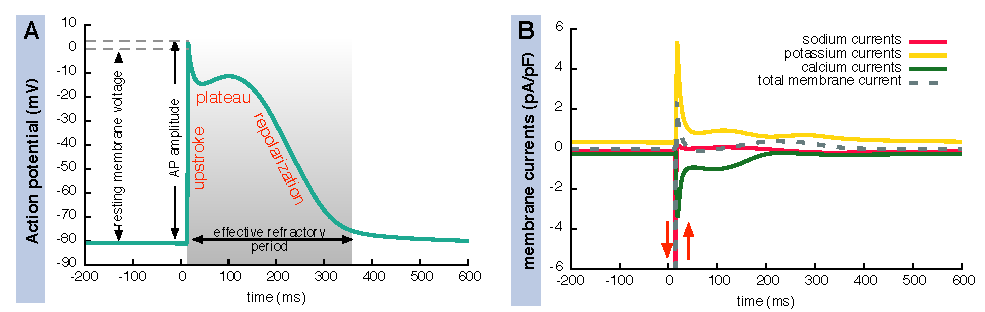
\includegraphics[width=\textwidth]{Funda-Med-AP}
 \caption{The course of the transmembrane voltage V$_\textnormal{m}$ during a cardiac \ac{AP} with its different phases (A) and the membrane currents carried by the different ions (B). The sodium current reaches an amplitude of $\approx$--70\,pA/pF. The calcium exchange with the sarcoplasmic reticulum is not considered. Courses were computed using the Courtemanche \etal model~\cite{courtemanche98}. Figure inspired by~\cite{schmidt10a}.}
 \label{fig:med:AP}
\end{figure}

\begin{figure}[ht]
\centering
\subfloat[Vector label (PDF format).]
	{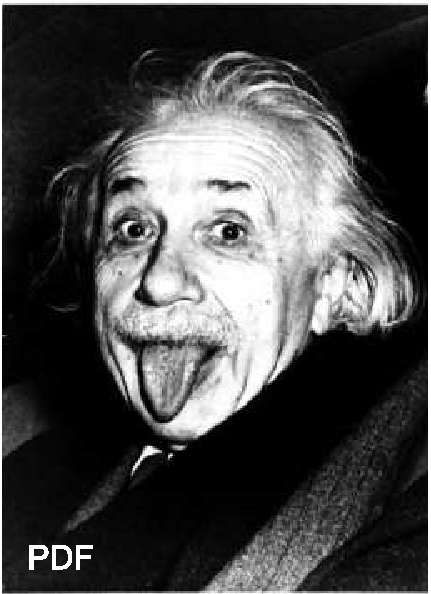
\includegraphics[width=0.4\textwidth]{einsteinlabelVEC}}
\hspace{0.05\textwidth}
\subfloat[Pixel label (PNG format).]
	{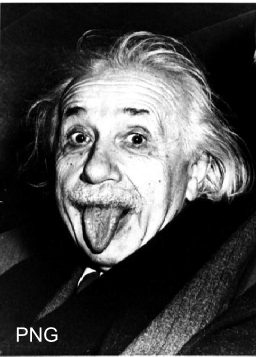
\includegraphics[width=0.4\textwidth]{einsteinlabelPIX}}
\caption{Photographs of different formats. One is vector~(a), one is pixel-base~(b).}
 \label{fig:med:einsteinComparsion}
\end{figure}

\Fig{fig:med:AP} is an example of a vector graphics figure. You can zoom in as you want, the figure will always stay sharp. This is the preferable format for all line drawings (\eg plots). Photographs are always saved as pixel graphics. However, labels can be added in a vector format (compare Figure~\ref{fig:med:einsteinComparsion}).\\
If you want to include a list of figures and a list of tables in your work, you probably want to provide short captions in square brackets as well. The

\clearemptydoublepage
%!TEX root = ../thesis.tex
\chapter{Mathematical Fundamentals}
\label{chap:mathFund}

Some mathematical formulas...\\
We establish the following transformations:
\begin{equation}
\label{eq:Fourier1}
F(u) = \frac{1}{N} \sum \limits_{x=0}^{N-1}f(x) e^{ -j 2 \pi \frac{u x}{N} }
  = \frac{1}{N} \sum \limits_{x=0}^{N-1}f(x) W_{N}^{ux}
\textrm{,}
\end{equation}
with $W_{N} = e^{ -j 2 \pi \frac{1}{N}} $ and $u=0,1,\dots,N-1$. Under the assumption of $N$ being..., \Eq{eq:Fourier1} can be expressed as...

\clearemptydoublepage

\ifthesisIsDiss  %Title
\part{Methods}
\fi

%!TEX root = ../thesis.tex
\chapter{Method A}
\label{chap:methA}

\section{Tables}
\label{sec:meth:tables}
Tables are a good way to present quantitative results. Mostly, they look best if you try to avoid vertical grid lines. \Tab{tab:meth:coverage} is an example of a table with a rather complex layout. \Tab{tab:meth:ionConcentrations} uses color to underline the structure and guide the eye. Decide for yourself what you like most and suits your needs best.
\begin{table}[tb]
\caption{Degree of coverage of RA elements with paths vulnerable to AFlut for different substrates and antiarrhythmic drugs. Some more description...}
\begin{center}
\begin{tabular}{lrrrcrrr}\toprule
& \multicolumn{7}{c}{\textbf{Degree of coverage}}\\ \cmidrule{2-8}
& \multicolumn{3}{c}{\textbf{Original CV}} & &\multicolumn{3}{c}{\textbf{Total activation time matched}} \\ \cmidrule{2-4} \cmidrule{6-8}
& no drug & amiodarone & dronedarone & & no drug & amiodarone & dronedarone \\ \midrule
\textbf{Control} & 18.1\% & 70.5\% & 0.0\% & & 18.1\% & 0.0\% & 0.0\% \\
\textbf{cAF} & 96.0\% & 96.3\% & 95.6\% & & 96.2\% & 96.1\% & 94.9\% \\
\textbf{N588K} & 93.2\% & 94.1\% & 0.0\% & & 93.0\% & 77.8\% & 0.0\% \\
\textbf{L532P} & 96.2\% & 96.5\% & 34.5\% & & 96.3\% & 96.0\% & 11.1\% \\
\bottomrule
\end{tabular}
\end{center}
\label{tab:meth:coverage}
\end{table}

\begin{table}[tb]
\caption[Ion concentrations and Nernst potential]{Typical concentrations and Nernst potentials of ions in a muscle cell.}
\centering
\begin{tabular}{>{\columncolor{lightBlue}}cccc}
  \toprule\rowcolor{lightBlue}
  \textbf{Ion}& \multicolumn{2}{c}{\textbf{Concentration ($mmol/kg\,H_2O$)}} & \textbf{Nernst}\\ \rowcolor{lightBlue}
  \textbf{type}& intracellular & extracellular & \textbf{potential} (mV)\\\rowcolor{lightBlue}
  \midrule
  $K^{+}$&\cellcolor{lightYellow} 4.5 &\cellcolor{lightYellow} 160 &\cellcolor{lightYellow} --95.4\\
  $Na^{+}$&\cellcolor{darkWhite} 144 &\cellcolor{darkWhite} 7 &\cellcolor{darkWhite} 80.2\\
  $Ca^{2+}$&\cellcolor{lightYellow} 1.3 &\cellcolor{lightYellow} 1e-5~to~1e-4 &\cellcolor{lightYellow} 126.5~to~157.3\\
  $Cl^{-}$&\cellcolor{darkWhite} 114 &\cellcolor{darkWhite} 7 &\cellcolor{darkWhite} --74.5\\
  \bottomrule
\end{tabular}
\label{tab:meth:ionConcentrations}
\end{table}


\section{Algorithms}
\label{sec:meth:algorithms}
\begin{algorithm}[tb]
\caption{The fast marching method. $\mathcal{N}\left(X\right)$ denotes the neighborhood of $X$.}
\begin{algorithmic}
\While{$TRIAL \neq\emptyset$}
  \State $X \gets \argmin_{X\in TRIAL}\left\{t_a\left(X\right)\right\}$
  \State $TRIAL \gets TRIAL\setminus\{ X\}$
  \State $KNOWN \gets KNOWN \cup \left\{ X \right\}$
  \ForAll{$\left(X_i \in \mathcal{N}\left(X\right) \right) \land \left( X_i \notin KNOWN \right)$}
    \State $t_a\left(X_i\right) \gets$ update$\left(X_i,X\right)$
    \If{$X_i \notin TRIAL$}
      \State $TRIAL \gets TRIAL \cup \left\{X_i\right\}$
    \EndIf
  \EndFor
\EndWhile
\end{algorithmic}
\label{alg:meth:fastMarching}
\end{algorithm}Algorithms in pseudo code can be defined using the \textit{algorithmicx} package: \url{https://www.ctan.org/tex-archive/macros/latex/contrib/algorithmicx/}. \Alg{alg:meth:fastMarching} gives an example.

\section{References}
\label{sec:meth:references}
To reference conveniently and consistently to chapters, sections, figures, tables, algorithms, equations and so on, we defined some macros:\\
\begin{itemize}
  \item In \Chap{chap:medFund}
  \item In \Sec{sec:anatomyPhysiology}..., in \Sec{sec:anatomyPhysiology:elphy}
  \item In \Fig{fig:med:AP}
  \item In \Tab{tab:meth:coverage}
  \item In \Alg{alg:meth:fastMarching}
  \item Under the assumption of equal anisotropy ratios, \Eq{eq:Fourier1} can be transformed into...
\end{itemize}

\subsection{Literature References}
\label{sec:meth:references:literature}
Regarding literature references, our reference management system \textit{refbase} already covers a good share of relevant literature. The \textit{refbase} entries are exported into a \textit{bibtex} file on the \textit{bordeaux} disk once every night: \textit{/Volumes/bordeaux/bibtex/export.bib}. In the template archive, there is a file \textit{refbase.bib} linking to the correct path on \textit{bordeaux}. References from there can be cited conveniently using the cite key, e.g.~\cite{courtemanche98}. When citing books, you should include the respective chapter~\cite[Chap. 5]{belytschko00} or pages  \cite[pp. 239--240]{belytschko00}. These specifications are not required when citing papers~\cite{riedel02} or preprints~\cite{schuler2021reducing}. You can switch between APA and IEEE citation style in \textit{config.tex}. If you need to preserve capital letters in reference titles (like for example ``ECG'' or if you cite German literature and write the thesis in English), you need to encapsulate these capital letters in curly braces (``{ECG}'') otherwise they will be converted to small letters.\\
The best way to include additional literature is directly import it to refbase as described in our wiki: \url{https://intern.ibt.uni-karlsruhe.de/wiki/Introduction_to_Refbase}.\\
At some point you probably want to change some things manually. The preferable way is to do so directly in \textit{refbase}. If this is not possible, you need a local bibtex file. As the \textit{refbase} export comprises several hundreds of thousands of lines and several megabytes, opening it in a text editor can be tedious and cumbersome. Therefore, we have a script \textit{ExtractBibEntriesFromBBL.pl} that extracts the entries you actually used and combines them in a new and smaller bibtex file (recommended name: \textit{reduced.bib}). You just need to pass the \textit{.bbl} file that is created during the compilation of your \LaTeX\ document using \textit{refbase.bib} (usually \textit{thesis.bbl}). Then, you can edit the entries in your local \textit{reduced.bib} file according to your needs. By putting curly braces around one or several characters, you can force them to be included in your references listing the way you defined them, \eg \{P\}-wave. You should do the \textit{ExtractBibEntriesFromBBL.pl} step towards the end of your writing when you feel that you won't include a lot more references. Running the script again will overwrite your local changes. Therefore, the easiest way to include additional references is to produce the bibtex entry right from the \textit{refbase} web interface and paste it into your local \textit{reduced.bib}.

\section{Abbreviations}
The acronym package helps you to keep track of abbreviations. See also \textit{abbreviations.tex} and \url{https://www.ctan.org/pkg/acronym}.
\cite{EKGO}

\clearemptydoublepage


\ifthesisIsDiss  %Title
\part{Results}
\fi

%!TEX root = ../thesis.tex
\chapter{Results}
\label{chap:results}
Please use title case for headings: \url{http://titlecapitalization.com}. If they are exceptionally long and do not fit within the header on normal text pages, please provide a short title as well as in this example:
\definecolor{mygray}{rgb}{0.5,0.5,0.5}
\lstset{
 basicstyle=\footnotesize,
 commentstyle=\color{mygray},
 keywordstyle=\color{blue},
 breaklines=true,
 frame=single,
 language=[LaTeX]TeX,
}
\begin{lstlisting}
\chapter{Ground Breaking Findings That Will Change
         the World and How We See It --- Part 1}
\markboth{Chapter \thechapter.~~~Ground Breaking Results 1}{Chapter \thechapter.~~~Ground Breaking Results 1}
\label{chap:findingsA}
\end{lstlisting}
If you want a shorter entry in the ToC as well, you can supply it in squared brackets:
\begin{lstlisting}
\chapter[Ground Breaking Results Changing the World Pt 1]{Ground Breaking Findings That Will Change the World and How We See It --- Part 1}
\markboth{Chapter \thechapter.~~~Ground Breaking Results 1}{Chapter \thechapter.~~~Ground Breaking Results 1}
\label{chap:findingsA}
\end{lstlisting}
The paragraphs above also serve as examples of how to include code. For details, see \eg \url{https://en.wikibooks.org/wiki/LaTeX/Source_Code_Listings}.


\clearemptydoublepage

%!TEX root = ../thesis.tex
\chapter{Discussion}
\label{chap:discussion}

Discuss your results here!


%!TEX root = ../thesis.tex
\chapter{Outlook}
\label{chap:outlook}

\clearemptydoublepage
%!TEX root = ../thesis.tex
\chapter{Conclusion}
\label{chap:conclusion}

\clearemptydoublepage

\begin{appendix}
% uncomment the following line if you want to hide Appendix sections from TOC
%\addtocontents{toc}{\protect\setcounter{tocdepth}{0}}
%!TEX root = ../thesis.tex
\chapter{Additional Stuff 1}
\label{app:stuff1}

Whatever is not important enough to be included in the main document body but too important to leave out completely.

\end{appendix}

\clearemptydoublepage
\backmatter
\chapterstyle{default}
\iflists
  \listoffigures
  \clearemptydoublepage
  \listoftables
  \clearemptydoublepage
\fi

% References
{
 \ifafive
  \footnotesize
  \setlength{\bibsep}{1pt}
 \else
  \small
  \setlength{\bibsep}{2pt}
 \fi
 \bibliography{reduced} % or refbase
 \clearemptydoublepage
}

\ifthesisIsDiss
  \include{Parts/13-publications}
  \clearemptydoublepage
\fi

\end{document}

